
\documentclass[12pt]{article}

% Layout.
\usepackage[top=1.0in, bottom=0.75in, left=1in, right=1in, headheight=1.0in, headsep=0pt]{geometry}

% Fonts.
\usepackage{mathptmx}
\usepackage[scaled=0.86]{helvet}
\renewcommand{\emph}[1]{\textsf{\textbf{#1}}}

% TiKZ.
\usepackage{tikz, pgfplots}
\usetikzlibrary{calc}
\pgfplotsset{my style/.append style={axis x line=middle, axis y line=
middle, xlabel={$x$}, ylabel={$y$}, axis equal }}

% Misc packages.
\usepackage{amsmath,amssymb,latexsym}
\usepackage{graphicx}
\usepackage{array}
\usepackage{xcolor}
\usepackage{multicol}
\usepackage{adjustbox}


% Commands to set various header/footer components.
\makeatletter
\def\doctitle#1{\gdef\@doctitle{#1}}
\doctitle{Use {\tt\textbackslash doctitle\{MY LABEL\}}.}
\def\docdate#1{\gdef\@docdate{#1}}
\docdate{Use {\tt\textbackslash docdate\{MY DATE\}}.}
\def\doccourse#1{\gdef\@doccourse{#1}}
\let\@doccourse\@empty
\def\docscoring#1{\gdef\@docscoring{#1}}
\let\@docscoring\@empty
\def\docversion#1{\gdef\@docversion{#1}}
\let\@docversion\@empty
\makeatother

% Headers and footers layout.
\makeatletter
\usepackage{fancyhdr}
\pagestyle{fancy}
\fancyhf{} % Clears all headers/footers.
\lhead{\emph{\@doctitle\hfill\@docdate}
\ifnum \value{page} > 1\relax\else\\
\emph{Name: \rule{3.5in}{1pt}\hfill \@docscoring}
\\
%\emph{Circle one: \quad Rhodes (F01) \hskip 1ex\rule{1pt}{9pt}\hskip 1ex Bueler (F02)}
\fi}

\rfoot{\emph{\@docversion}}
\lfoot{\emph{\@doccourse}}
\cfoot{\emph{\thepage}}
\renewcommand{\headrulewidth}{0pt}%
\makeatother

% Paragraph spacing
\parindent 0pt
\parskip 6pt plus 1pt

% A problem is a section-like command. Use \problem{5} to
% start a problem worth 5 points.
\newcounter{probcount}
\newcounter{subprobcount}
\setcounter{probcount}{0}
\newcommand{\problem}[1]{%
\par
\addvspace{4pt}%
\setcounter{subprobcount}{0}%
\stepcounter{probcount}%
\makebox[0pt][r]{\emph{\arabic{probcount}.}\hskip1ex}\emph{[#1 points]}\hskip1ex}
\newcommand{\thesubproblem}{\emph{\alph{subprobcount}.}}

% Subproblems are an enumerate-like environment with a consistent
% numbering scheme. 
% Use \begin{subproblems}\item...\item...\end{subproblems}
\newenvironment{subproblems}{%
\begin{enumerate}%
\setcounter{enumi}{\value{subprobcount}}%
\renewcommand{\theenumi}{\emph{\alph{enumi}}}}%
{\setcounter{subprobcount}{\value{enumi}}\end{enumerate}}

% Blanks for answers in normal and math mode.
\newcommand{\blank}[1]{\rule{#1}{0.75pt}}
\newcommand{\mblank}[1]{\underline{\hspace{#1}}}
\def\emptybox(#1,#2){\framebox{\parbox[c][#2]{#1}{\rule{0pt}{0pt}}}}

% Misc.
\renewcommand{\d}{\displaystyle}
\newcommand{\ds}{\displaystyle}
\def\bc{\begin{center}}
\def\ec{\end{center}}

\newcommand{\ans}[1][2]{ \ \rule{#1 in}{.5 pt} \ }


\doctitle{Math 251: Quiz 7}
\docdate{October 29, 2019}
\doccourse{UAF Calculus I}
\docversion{v-1}
\docscoring{{\Large \strut}\blank{0.8in} / 25}

\begin{document}
25 points possible.  No aids (book, calculator, etc.) are permitted.  You need not simplify, but show all work and use proper notation for full credit.

% like 4.1 #5,6;  note #5 is on WebAssign
\problem{4}  Use the graph to determine all the \underline{absolute} and \underline{local} maximum and minimum values of the function. If a value does not exist, write DNE.

\begin{adjustbox}{valign=t,minipage={.45\textwidth}}
{\renewcommand{\arraystretch}{2.5}
\begin{tabular}{p{1.2in} || p{.5in}| p{.5in}}
& {\bf $y$-value} & {\bf occurs at $x =$}\\ \hline
local max (list all) &\vspace{1in} &  \\ \hline
local min (list all) & \vspace{1in} & \\ \hline
absolute max& &\\ \hline
absolute min & & \\ \hline
\end{tabular}
}
\end{adjustbox}
%
\begin{adjustbox}{valign=t,minipage={.45\textwidth}}
 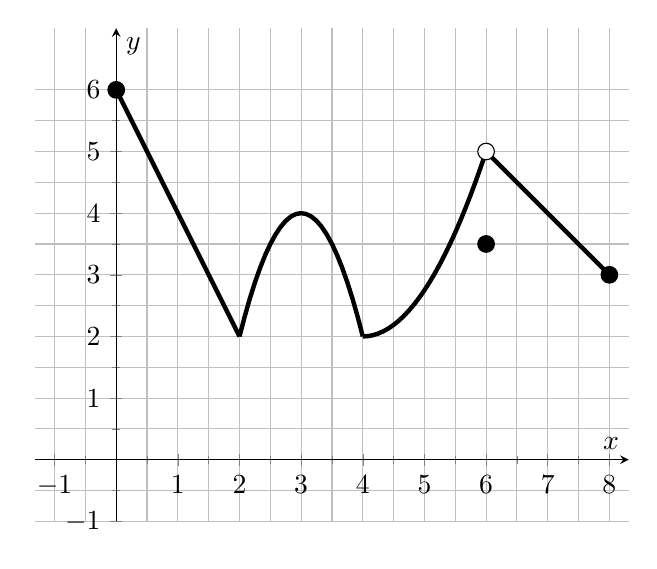
\begin{tikzpicture}
\begin{axis}[scale=1.1, my style, xtick={-1,0,...,8}, ytick={-1,0,...,6},
xmin=0, xmax=7, ymin=-1, ymax=7, grid=both, minor y tick num=1,
        minor x tick num=1, mark size=3.0pt]
\addplot[domain=0:2,ultra thick] { (6-2)/(0-2)*(x-0)+6};
\addplot[domain=2:4, ultra thick] {-2*(x-2)*(x-4)+2};
%\addplot[domain=4:6, ultra thick] {2.+(x-4)^{2}};
\addplot[domain=4:6, ultra thick] {2+.75*(x-4)^2};
\addplot[domain=6:8, ultra thick] {(5-3)/(6-8)*(x-6)+5};
\addplot[mark=*,only marks] coordinates {(0,6)(8,3)(6,3.5)};
\addplot[mark=*,fill=white,only marks] coordinates {(6,5)};
\end{axis}
\end{tikzpicture}
\end{adjustbox}

%\vspace{10mm}

% like 4.1 #48
\problem{7} Find the absolute maximum and absolute minimum values of 
\[f(x) = x^{3}+3x^{2}-9x-3 \]
 on the interval $[0,3]$, and the $x$-values where they occur.
    
\vfill

\hfill Absolute Maximum: $y =$ \ans[1] at $x = $\ans[1]

\hfill Absolute Minimum: $y =$ \ans[1] at $x = $\ans[1]

\newpage
\problem{8} %Suppose $f$ is continuous on $[0,4]$ and has a derivativeat each point in $(0,4)$.  Suppose $f(0)=5$ and $f(4)=-1$. 

Consider the function $f(x)$ % = (x-1)^{3}+1$ 
shown on the graph below, on the interval $[0,2]$. It has the property that $f(0) = 0$ and $f(2) = \frac{3}{2}$.

\begin{adjustbox}{valign=t,minipage={.45\textwidth}}
\begin{subproblems}
\item Fill in the blanks: The function $f(x)$ satisfies the hypotheses of the Mean Value Theorem, which means that $f(x)$ is \ans[2] \\
and \ans[2].


\item What can we conclude about the function $f(x)$, by the Mean Value Theorem? (That is, state the conclusion of the Mean Value Theorem, specified to this function.) 
\vskip 1in
\end{subproblems}
\end{adjustbox}
%\vskip 1in
\begin{adjustbox}{valign=t,minipage={.45\textwidth}}
\begin{subproblems}
\item The graph of $f(x)$ is shown below. \fbox{Add lines to the graph} to illustrate what the Mean Value Theorem says about this function. Then use the the graph to estimate the value(s) of $c$ whose existence is predicted by the Mean Value Theorem.

%\begin{center}
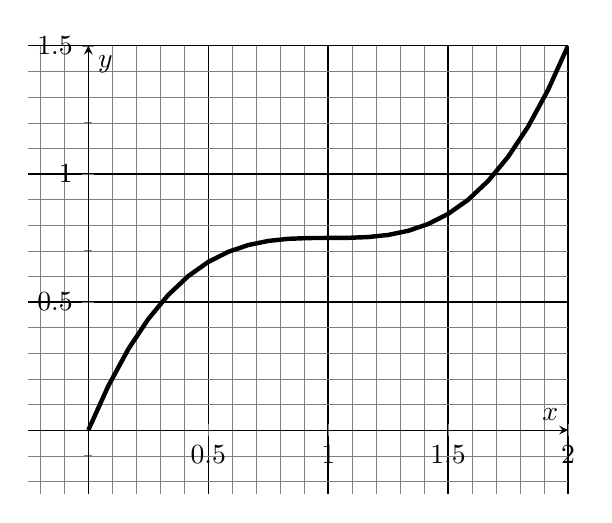
\begin{tikzpicture}
\begin{axis}[scale = 1, 
axis x line=middle, axis y line=
middle, xlabel={$x$}, ylabel={$y$}, %xtick={-1,-1/2,0,1/2,1,1.5,2}, 
%ytick={-1,0,1,2,3,4,5,6}, 
xmin=-0.25, xmax=2.0, ymin=-0.25, ymax=1.5, grid=both, minor y tick num=4,
        minor x tick num=4,
        grid style={line width=.1pt, draw=black!50},
    major grid style={line width=.5pt,draw=black},
        ]
\addplot[domain=0:2, ultra thick]{3/4*((x-1)*(x-1)*(x-1)+1)};
%\addplot[domain=0:2, dashed]{( ((3-1)*(3-1)*(3-1)+1) - ((0-1)*(0-1)*(0-1)+1))/(3-0 )(x-0)+(0) };
\end{axis}

\end{tikzpicture}

 Estimated value(s) (to the nearest tenth) of $c$ predicted by MVT (list all): \ans[3]
 \end{subproblems}
 \end{adjustbox}
%\end{center}


% like 4.1 #43
\problem{6} Find the critical numbers (critical points) of the function
  \[g(x) = \sqrt[3]{x^{2} - 9}. \]

\vfill

\hfill Critical points: $x = $\ans

\end{document}